% vim: spell spelllang=en:
\documentclass[12pt, oneside]{article}
\usepackage[a4paper, left=2.5cm, right=2.5cm, top=2.5cm, bottom=2.5cm]{geometry}

\usepackage[utf8]{inputenc} % Use unicode
\usepackage[T1]{fontenc}
\usepackage[english]{babel} % Names in spanish

%% Bibliography:
%\usepackage{comment}
%\usepackage[
    %backend=biber,
    %style=numeric,
%]{biblatex}
%\DeclareNameAlias{default}{last-first}

%\usepackage{csquotes}       % For bibliography quotations
%\DeclareQuoteAlias{spanish}{catalan}

%\addbibresource{biblio.bib}
%% see:
%% https://www.sharelatex.com/learn/Bibliography_management_in_LaTeX#The_bibliography_file

%\usepackage{datetime} % Customize date
%% \monthyeardate\today gives the date without the day
%\newdateformat{monthyeardate}{%
    %\monthname[\THEMONTH], \THEYEAR}

% For cross references
\usepackage[colorlinks = true]{hyperref}
\usepackage[catalan]{varioref}
%\usepackage{cleveref}
%hyperref configuration so that it doesn't contrast so much colorlinks,
\hypersetup{
   linkcolor={black},
   citecolor={black},
   %linkcolor={red!50!black},
   %citecolor={blue!50!black},
   urlcolor={blue!80!black}
}

\usepackage{xcolor}     % color

\usepackage{mathtools}  % amsmath + more
\usepackage{amsthm}     % Theorem enviroment
\usepackage{amssymb}    % More symbols
\usepackage{amstext}    % Text inside mathenv

\usepackage{relsize}    % Bigger math with mathlarger{___}
\usepackage{nicefrac}   % nice fractions in one line

\usepackage[export]{adjustbox}  % Adjust table size
\usepackage{float}              % Force tables and images position (H and H!)
\usepackage{wrapfig}            % Wrap images like in HTML

\usepackage{tabularx, colortbl, booktabs}    % Better tables
\usepackage{longtable}                      % Multiple page table

% Split cell in lines and more formating options inside table
\usepackage{array, multirow, multicol, makecell}

%\usepackage{subcaption}                     % Subfigures
%\usepackage[framemethod=tikz]{mdframed}     % Custom frames

%\usepackage[bottom]{footmisc} % Footnotes at bottom of page

%\usepackage[alsoload=hep]{siunitx}          % SI units and uncertainties
%\sisetup{locale = FR}                       % Commas and so on for spanish
%\sisetup{separate-uncertainty=true}
%\sisetup{
  %per-mode=fraction,
  %fraction-function=\nicefrac
%}

%\usepackage{tikz}
%%\usetikzlibrary{arrows}
%%\usetikzlibrary{scopes}
%\usetikzlibrary{babel}

%\usepackage{listings}       % For code blocks

%% Custom code highlight
%\definecolor{codegreen}{rgb}{0,0.6,0}
%\definecolor{codegray}{rgb}{0.5,0.5,0.5}
%\definecolor{codepurple}{rgb}{0.58,0,0.82}
%\definecolor{backcolour}{rgb}{0.95,0.95,0.92}
%\definecolor{lightblue}{RGB}{135,206,250}

%\lstdefinestyle{mystyle}{ backgroundcolor=\color{backcolour},
    %commentstyle=\color{codegreen}, keywordstyle=\color{blue},
    %numberstyle=\tiny\color{codegray}, stringstyle=\color{red},
    %identifierstyle=\color{black}, basicstyle=\footnotesize,
    %%breakatwhitespace=false,
    %breaklines=true,
    %%captionpos=b,                    keepspaces=true,
    %numbers=left,                    numbersep=5pt,
    %showspaces=false,
    %%showstringspaces=false, showtabs=false,
    %tabsize=4
%}
%\lstset{style=mystyle}

\newcommand{\whitepage}{
    \clearpage\thispagestyle{empty}\addtocounter{page}{-1} \newpage \clearpage
}

% Add command before appendix session for page numbering: A-1
%\newcommand{\appendixpagenumbering}{
    %\break
    %\pagenumbering{arabic}
    %\renewcommand{\thepage}{\thesection-\arabic{page}}
%}

%% Custom Math operators (functions not in italic in math mode):
%\DeclareMathOperator{\arcsec}{arcsec}
%\DeclareMathOperator{\arccot}{arccot}
%\DeclareMathOperator{\arccsc}{arccsc}
%\DeclareMathOperator{\cis}{cis}


\usepackage[justification=centering]{caption}
\usepackage{subcaption}
\usepackage{graphicx}
\usepackage{enumitem}
\usepackage{lipsum}

\usepackage{siunitx}
\usepackage{hyphenat}

\usepackage{xcolor}

\definecolor{LightGray}{rgb}{0.83, 0.83, 0.83}
\definecolor{bg}{HTML}{282828}

\usepackage[newfloat]{minted}
\captionsetup[listing]{position=top}

\graphicspath{{figures/}}

\setminted{
style=monokai,
%frame=lines,
framesep=2mm,
baselinestretch=1.2,
breaklines,
bgcolor=bg,
fontsize=\footnotesize,
linenos
}

\renewcommand\theadfont{\bfseries}

\title{
    PAR Laboratory Assignment\\
    Lab 5: Geometric (data) decomposition: \\
    heat diffusion equation
}

\author{
    par2109:
    Aleix Boné,
    Alex Herrero
}

\date{
    Spring 2019-20
}

\begin{document}

\thispagestyle{empty}
\clearpage
\setcounter{page}{-1}

\begin{titlepage}
{%
    \centering
    \null{}
    \vfill
    {\Huge \bfseries PAR Laboratory Assignment\par}
    \vspace{3em}
    {\Large {\scshape Lab 5:} 
    Geometric (data) decomposition: \\
    heat diffusion equation
\par}
    \vfill
\begin{center}
\end{center}
    \vspace{3cm}

    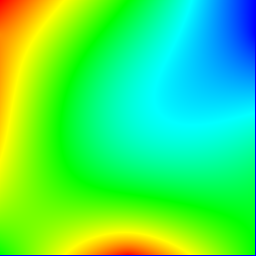
\includegraphics{images/jacobi}

    \vfill
    {\raggedleft{} \Large
        Aleix Boné\\
        Alex Herrero\\
        {\bfseries\ttfamily par2109}\\
        \vspace{4em}
        2020-06-05 % chktex 8
        \par}
}
\end{titlepage}

\tableofcontents
\pagebreak

\section{Introduction}%
\label{sec:introduction}

In this session we are going to work on the parallelization of a sequential code that
simulates heat diffusion in a solid body using two different solvers for the heat equation.
The program reads a configuration file that specifies the maximum number of steps, the size
of the body and the solver to use which can be either \emph{Jacobi} or \emph{Gauss-Seidel}.

The two solvers have different numerical properties and behave differently when parallelized.
With the \emph{Jacobi} method, the values of the \emph{i}th iteration remain unchanged until
the next iteration has been calculated, with Gauss-Seidel the results are used immediately.
Moreover, Gauss-Seidel converges faster than Jacobi.
\footnote{\url{https://www3.nd.edu/~zxu2/acms40390F12/Lec-7.3.pdf}}.

When we tried the sequential version of the program with the input in \texttt{test.dat}
we obtained different results as shown in figure~\ref{fig:mosaic_label} and 
\emph{Gauss-Seidel} was more than twice as fast than \emph{Jacobi}:

\begin{verbatim}
Iterations        : 25000
Resolution        : 254
Algorithm         : 1 (Gauss-Seidel)
Num. Heat sources : 2
   1: (0.00, 0.00) 1.00 2.50 
   2: (0.50, 1.00) 1.00 2.50 
Time: 2.394 
Flops and Flops per second: (8.806 GFlop => 3679.06 MFlop/s)
Convergence to residual=0.000050: 12409 iterations

Iterations        : 25000
Resolution        : 254
Algorithm         : 0 (Jacobi)
Num. Heat sources : 2
   1: (0.00, 0.00) 1.00 2.50 
   2: (0.50, 1.00) 1.00 2.50 
Time: 4.819 
Flops and Flops per second: (11.182 GFlop => 2320.50 MFlop/s)
Convergence to residual=0.000050: 15756 iterations
\end{verbatim}

% Sequential heat diffusion program
% differences between jacobi and gauss images

\begin{figure}[H]
    \centering
    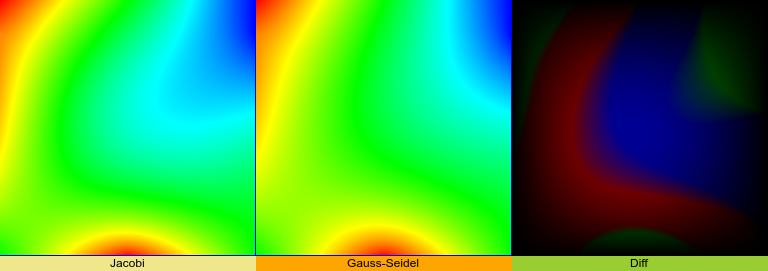
\includegraphics[width=0.8\linewidth]{images/mosaic_label}
    \caption{Comparison between heat map generated by Jacobi and Gauss-Seidel}%
    \label{fig:mosaic_label}
\end{figure}

\pagebreak
\section{Analysis of task granularities and dependences with \emph{Tareador}}%
\label{sec:analysis_of_task_granularities_and_dependences_with_tareador}

% dependency: sum on both jacobi and gauss

\begin{figure}[H]
    \begin{minipage}{0.5\textwidth}
    \centering
    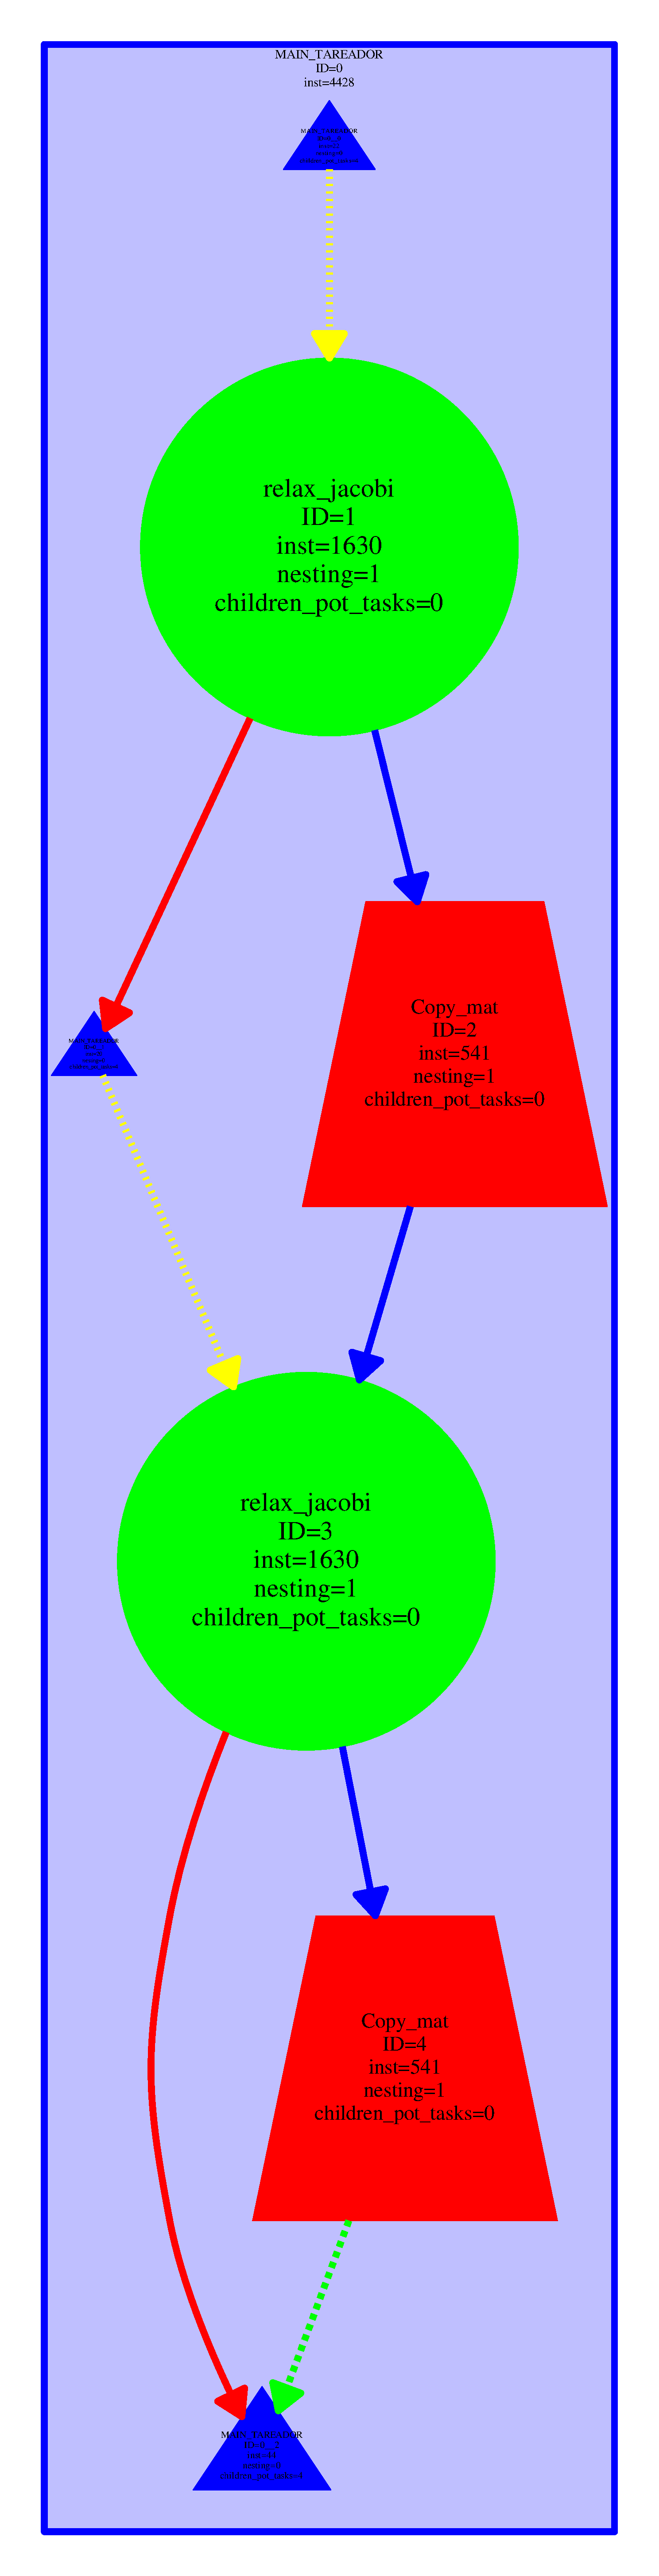
\includegraphics[width=0.2\linewidth]{dependency_coarse_jacobi}
    \caption{Coarse dependency graph of Jacobi}%
    \label{fig:dependency_coarse_jacobi}
    \end{minipage}
    \begin{minipage}{0.5\textwidth}
    \centering
    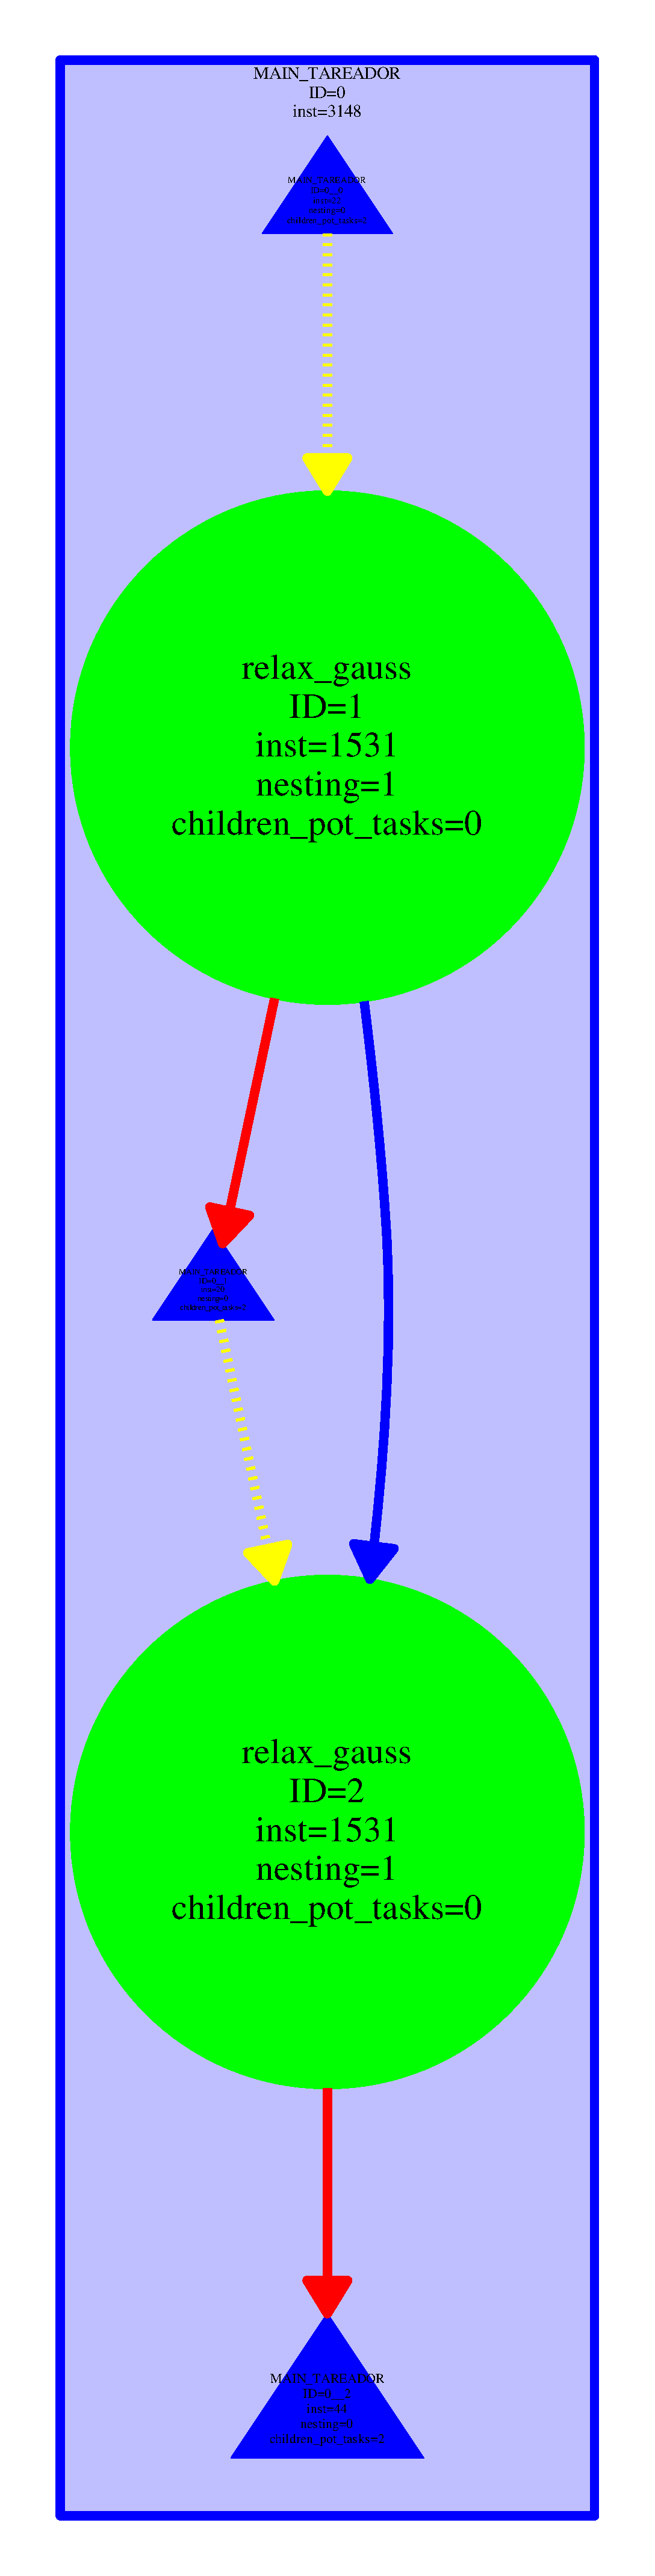
\includegraphics[width=0.2\linewidth]{dependency_coarse_gauss}
    \caption{Coarse dependency graph of Gauss-Seidel}%
    \label{fig:dependency_coarse_gauss}
    \end{minipage}
\end{figure}

Figures~\ref{fig:dependency_coarse_jacobi} and \ref{fig:dependency_coarse_gauss}
show the dependency graph obtained with \emph{tareador} for Jacobi and Gauss-Seidel
respectively (with very coarse granularity).

The first thing we notice is that there are two executions of
\texttt{relax\_jacobi} and \texttt{relax\_gauss}.  Taking a look at the code
shown in listing~\ref{lst:heat_while} we can see that the program applies the
relax function on the data until the residual obtained is small enough or the
maximum number of iterations is reached. Each iteration depends on the results
of the previous one, so they cannot be parallelized. In the case ran by
\emph{tareador} this is barely noticeable since the data used is very small and
the maximum number of iterations is set 2 with a resolution of 4. However for
\texttt{test.dat} the maximum number of iterations is set to 2500 with a resolution
of 254.

In the case of Jacobi there is also the function \texttt{copy\_mat} that is
used as an auxiliary matrix, since Jacobi does not modify \texttt{u} in place
and Gauss-Seidel does.  In fact, this is the main difference between the two
algorithms, Jacobi uses the matrix from the previous iteration of the method
while Gauss-Seidel uses modifies it as it traverses the matrix.

\begin{listing}[H]
\caption{heat.c}%
\label{lst:heat_while}
\inputminted[firstline=83,lastline=104]{c}{code/heat.c}
\end{listing}

In order to further analysis the potential parallelization of both both methods,
we have to look into the inner workings of each step of the relax functions. To
achieve this, we added finer \emph{tareador} task definitions, defining tasks
for each iteration of the loops as shown in Listing~\ref{lst:solver-tar}:

\begin{listing}[H]
\caption{soler-tareador.c}%
\label{lst:solver-tar}
\inputminted[firstline=28,lastline=43]{c}{code/solver-tareador.c}
\vspace{-2.5em}
\inputminted[firstline=56,lastline=72]{c}{code/solver-tareador.c}
\end{listing}

\begin{figure}[H]
    \begin{minipage}{0.5\textwidth}
        \centering
        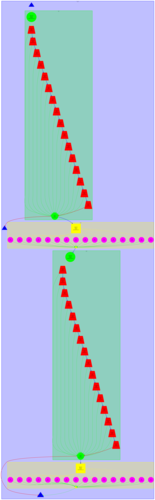
\includegraphics[height=6cm]{dependency_fine_jacobi.png}
        \caption{Fine dependency graph \\ Jacobi}%
        \label{fig:dependency_fine_jacobi}
    \end{minipage}
    \begin{minipage}{0.5\textwidth}
        \centering
        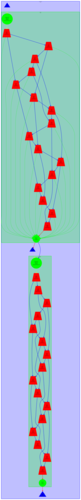
\includegraphics[height=6cm]{dependency_fine_gauss.png}
        \caption{Fine dependency graph \\ Gauss-Seidel}%
        \label{fig:dependency_fine_gauss}
    \end{minipage}
\end{figure}

Figure~\ref{fig:dependency_fine_jacobi} and~\ref{fig:dependency_fine_gauss} show the
task dependency graph obtained with \emph{tareador}. The results are disappointing, since
there are dependencies making all the code sequential, nevertheless, if we look at the
variables causing those dependencies (shown in figures~\ref{fig:dependence_jacobi}
and~\ref{fig:dependence_gauss}) we see that the dependence in both cases is caused by
the \texttt{sum} variable which in this case is only used once and can be reduced or
protected by an atomic clause. This means that we can still parallelize most of the
work.

However in the case of Gauss-Seidel there is another dependency corresponding to some
memory positions in the heap, which by analyzing the code we can determine that this
data on the heap is the matrix \texttt{u}. Since Gauss-Seidel modifies the data in
\texttt{u}, this creates a dependency between iterations of the method. More specifically
they have a dependency on the left cell and the top cell of the matrix.

\begin{figure}[H]
    \begin{minipage}{0.5\textwidth}
        \centering
        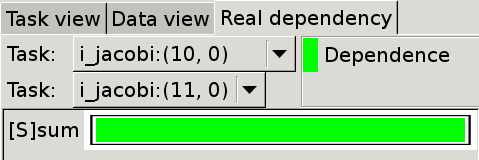
\includegraphics[width=0.9\linewidth]{dependence_jacobi}
        \caption{Task dependence \\ Jacobi}%
        \label{fig:dependence_jacobi}
    \end{minipage}
    \begin{minipage}{0.5\textwidth}
        \centering
        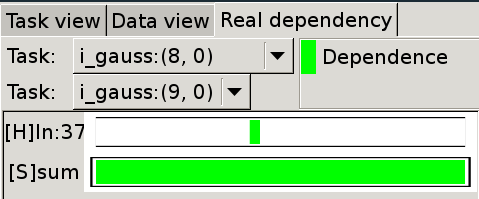
\includegraphics[width=0.9\linewidth]{dependence_gauss}
        \caption{Task dependence \\ Gauss-Seidel}%
        \label{fig:dependence_gauss}
    \end{minipage}
\end{figure}

In figure~\ref{fig:dependency_fine_jacobi_nosum} and~\ref{fig:dependency_fine_gauss_nosum}
we show the data decomposition obtained with \emph{tareador} ignoring the \texttt{sum} variable
dependency.
We can see that if we eliminate the sum dependency in Jacobi the iterations of the
loop inside \texttt{relax\_jacobi} are embarrassingly parallel. With Gauss-Seidel,
we can clearly see the top-left dependency of the iterations caused by the modification
of the matrix \texttt{u}.

\begin{figure}[H]
    \begin{minipage}{0.5\textwidth}
        \centering
        \includegraphics[height=6cm]{dependency_fine_jacobi_nosum}
        \caption{Fine dependency graph \\ Jacobi (no sum)}%
        \label{fig:dependency_fine_jacobi_nosum}
    \end{minipage}
    \begin{minipage}{0.5\textwidth}
        \centering
        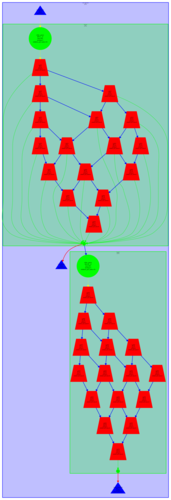
\includegraphics[height=6cm]{dependency_fine_gauss_nosum}
        \caption{Fine dependency graph \\ Gauss-Seidel (no sum)}%
        \label{fig:dependency_fine_gauss_nosum}
    \end{minipage}
\end{figure}

\pagebreak
\section{OpenMP parallelization and execution analysis: \emph{Jacobi}}

\begin{listing}[H]
    \caption{solver.c}%
    \label{lst:solver-omp}
    \inputminted[firstline=17,lastline=39]{c}{code/solver-omp-orig.c}
\end{listing}

If we examine \texttt{solver.c} (listing~\ref{lst:solver-omp} we see that there are some differences 
from the \emph{tareador} version,
mainly that there is an additional outer for loop that is repeated \texttt{howmany} times and determines the
range of the \texttt{i} variable of the first \texttt{for}. If we look at what \texttt{lowerb} and
\texttt{upperb} (listing~\ref{lst:heat_h}) we can see that they compute the index bounds of the block
number \texttt{id} if there are \texttt{n} indices divided in \texttt{p} blocks.

The code splits the matrix in \texttt{howmany} (in this case 4) blocks of rows and computes them.
We decided to use this division as a basis for our OpenMP implementation.

\begin{listing}[H]
    \caption{heat.h \texttt{\#define}}%
    \label{lst:heat_h}
    \inputminted[firstline=59,lastline=61]{c}{code/heat.h}
\end{listing}


\begin{figure}[H]
    \centering
    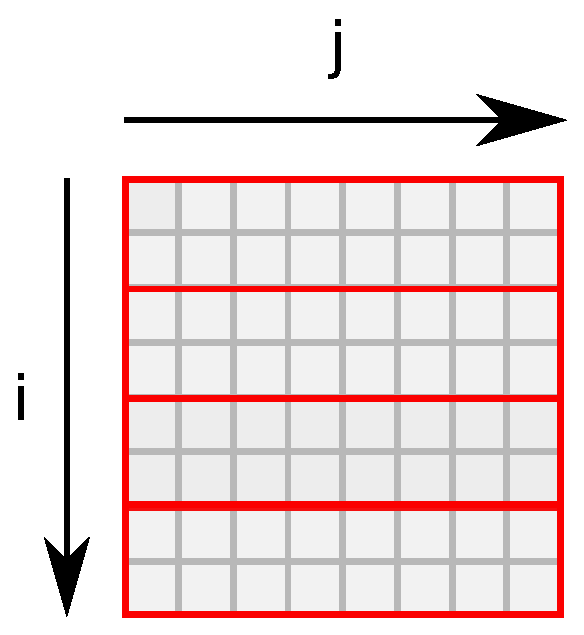
\includegraphics[width=0.3\textwidth]{jacobi_blocks}
    \caption{Jacobi row block division with 4 threads on a 8x8 matrix}%
    \label{fig:blocks-jacobi}
\end{figure}

Figure~\ref{fig:blocks-jacobi} shows an example of the block division by rows performed on a 8x8 matrix
with 4 threads. In cases where the number of threads does not divide the dimension of the matrix, the final
block would be smaller to make up the difference.

As we discussed on the \emph{tareador} analysis, the only dependency between tasks is the variable
\texttt{sum}, so to guarantee that there are no data races we must apply a reduction. Given that we cannot use
the \texttt{pragma omp for} directives, we decided to create a variable \texttt{sum\_tmp} private on each
task to store the sum of each task and then perform an atomic addition to \texttt{sum} at the end of the tasks.
We also added \texttt{private(diff)} and \texttt{firstprivate(blockid)} since they where declared before the
task (blockid has to be firstprivate since the value is needed).
Listing~\ref{lst:jacobi_first} shows the first version of our code 

\begin{listing}[H]
    \caption{solver-omp.c Initial OpenMP version of jacobi method}%
    \label{lst:jacobi_first}
    \inputminted[firstline=26,lastline=55]{c}{code/solver-omp-jacobi-v1.c}
\end{listing}

Our initial version of the code did not modify the variable \texttt{howmany} which meant that we always
divided the matrix in 4 blocks which is not optimal since if we have more than 4 threads there are threads
that are not doing any work. This can be seen in the paraver trace we generated and that we show in
figure~\ref{fig:trace-jacobi0} where we can see that there are always 4 concurrent tasks and 4 threads are unused.

We also noticed that there where huge sequential versions, which were caused by the matrix copy operation.
In our analysis with \emph{tareador} we saw that there were no dependencies between loop iterations so
we decided to parallelize it to remove this bottleneck. Our first approach, which was quite naive, was to
assign a task to every iteration of the loop, however the code run much slower than the sequential
version due to the massive overhead of the task creation, we decided to use the same geometric data
decomposition used in the jacobi function.

\begin{figure}[H]
    \centering
    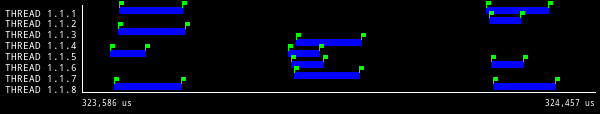
\includegraphics[width=0.8\textwidth]{jacobi_0_tasks}
    \caption{Parallel tasks Jacobi}%
    \label{fig:trace-jacobi0}
\end{figure}

Listing~\ref{lst:jacobi} shows the improved version of \emph{Jacobi} with improvements on \texttt{copy\_mat}
and jacobi. We removed the outer \texttt{for}
since is not needed as we use the parallel region with all its threads to divide the matrix. We also
applied the same division and parallelization approach to the \texttt{copy\_mat} function.
In figure~\ref{fig:trace-jacobi1} we can see the improvement over the previous version and how this time
there are much more tasks and all threads are used in parallel, although some have more work than others.

\begin{figure}[H]
    \centering
    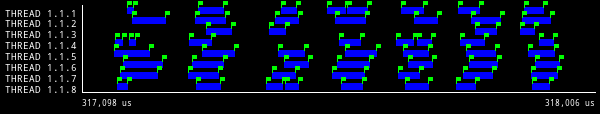
\includegraphics[width=0.8\textwidth]{jacobi_1_tasks}
    \caption{Parallel tasks jacobi improved}%
    \label{fig:trace-jacobi1}
\end{figure}

\begin{listing}[H]
    \caption{solver-omp.c Improved jacobi}%
    \label{lst:jacobi}
    \inputminted[firstline=8,lastline=19]{c}{code/solver-omp.c}
    \vspace{-2.5em}
    \inputminted[firstline=25,lastline=52]{c}{code/solver-omp.c}
\end{listing}

In figure~\ref{fig:strong-jacobi} we can see the time and speed-up plots for different number 
of OMP threads of the improved version.
We can see that the execution time goes from ~5 seconds to less than 1 second
achieving a very good speed-up till around 9 threads, this is probably caused by the task creation
overhead.

\begin{figure}[H]
    \centering
    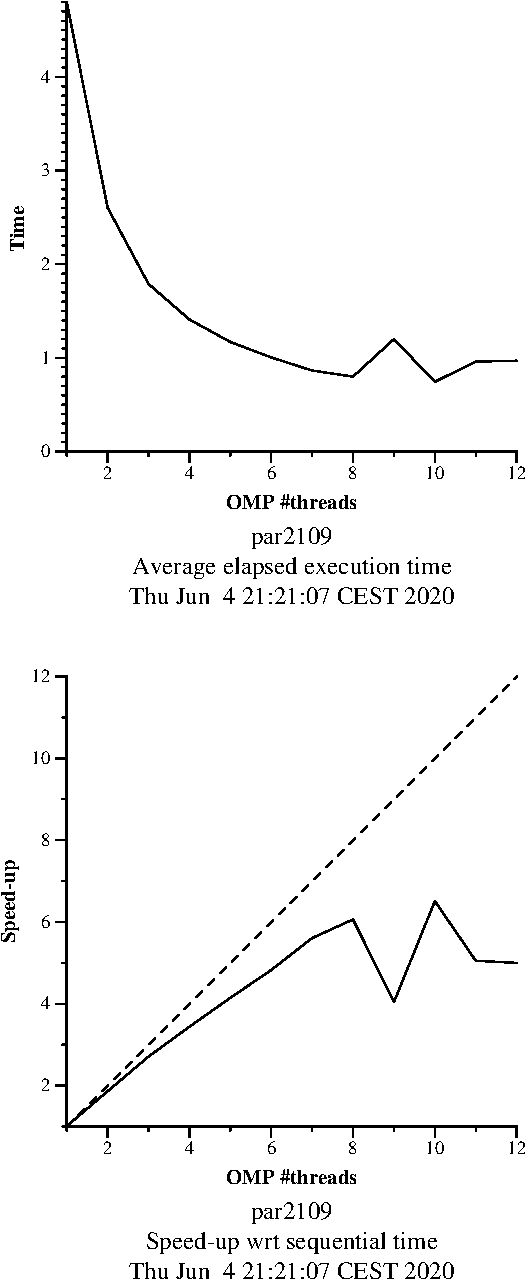
\includegraphics[width=0.3\textwidth]{heat-omp-strong-jacobi-crop}
    \caption{Strong scalability graph \\ Jacobi}%
    \label{fig:strong-jacobi}
\end{figure}


% TODO: dibujo de matriz

\pagebreak
\section{OpenMP parallelization and execution analysis: \emph{Gauss-Seidel}}

\begin{listing}[H]
    \caption{solver.c}%
    \label{lst:solver-omp-GS}
    \inputminted[firstline=44,lastline=66]{c}{code/solver-omp-orig.c}
\end{listing}

\begin{listing}[H]
    \caption{solver-omp-gauss.c}%
    \label{lst:solver-omp-gauss}
    \inputminted[firstline=57,lastline=89]{c}{code/solver-omp.c}
\end{listing}

% Describe how did you implement the parallelization strategy for the Gauss-Seidel solver and how did you guarantee the proper synchronization between threads.

% QUIERO LLORAR LLEVO UNA HORA DELANTE DEL ORDENADOR SIN ESCRIBIR UNA SOLA PALABRA...
% F

For implementing the parallelization strategy for the Gauss-Seidel solver we had to add two loops, for the rows and columns.


A row or column based decomposition would not work in this case, since as we have seen in the
tareador analysis, each iteration depends on the value of the previous row and column,
which means that if we implemented it like that the resulting code would be sequential.

The best approach is to divide the matrix in blocks and define the dependencies between the
iterations using. Figure~\ref{fig:block-gauss} shows an example
of the block decomposition and the dependencies in blue. For the task corresponding to
the block $i,j$ to begin executing, it must wait for both $i-1, j$ and $i, j-1$ to finish.
This kind of restriction can be defined using \texttt{}

% hello? hi
% hmmmmmmm, no falta un sink?
%ahora meacabo de drogar, a ver si ahora me concentro mas

\begin{figure}[H]
    \centering
    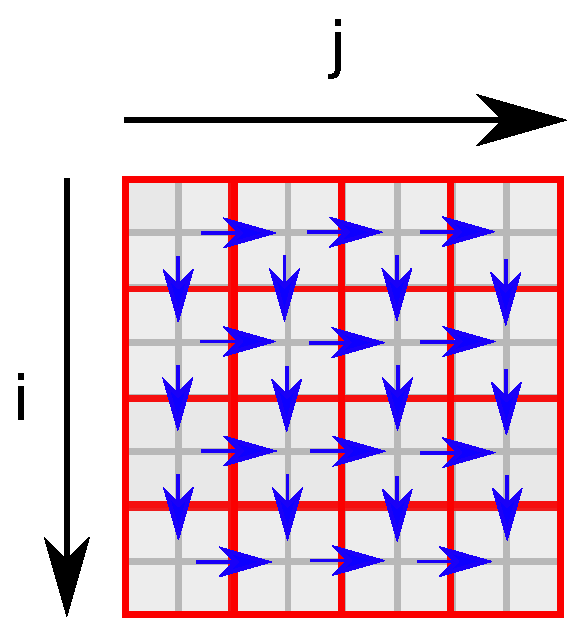
\includegraphics[width=0.3\textwidth]{gauss_blocks}
    \caption{Gauss block decomposition with 4 threads on a 8x8 matrix}%
    \label{fig:blocks-gauss}
\end{figure}


% Analyse the speed–up (strong scalability)plot that has been obtained for the different numbers of processors, reasoning about the performance that is observed 
% TODO: and including captures of Paraver windows to justify your explanations.

\begin{figure}[H]
    \centering
    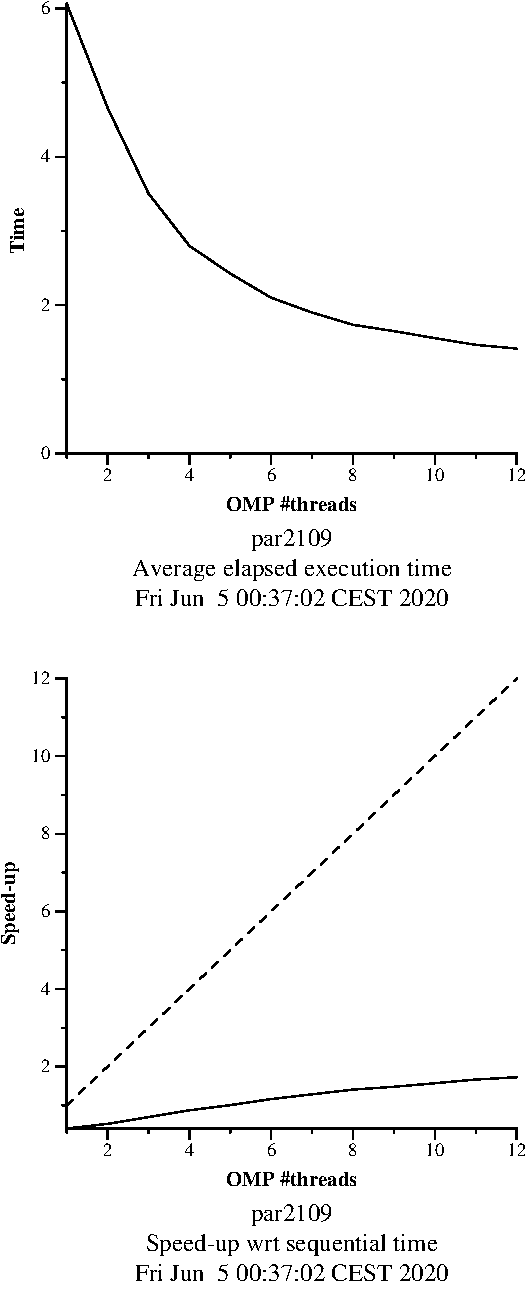
\includegraphics[width=0.3\textwidth]{heat-omp-strong-gauss-crop}
    \caption{Strong scalability graph \\ Gauss}%
    \label{fig:strong-gauss}
\end{figure}

As in the previous section, in figure~\ref{fig:strong-gauss} we can see the time and speed-up plots for different number 
of OMP threads, but in this case, of the execution of the Gauss-Seidel solver. We can observe how the execution time improves with the number of threads, and the speed-up gets better. But, as we can see, the speed-up is not even close to the ideal speed-up line, and that is because of the difference between the synchronization and computation for each thread, and that depends on the size of the block.

% Finally explainhow did you obtain the optimum value for the ratio computation/synchronization in the parallelization of this solver for 8 threads.

% esto nose mucho, pero bueno. He provado cambiando howmany un poco y con 16 me iba un poco mejor que con el resto.,...

We tried changing the value of \texttt{howmany} and surprisingly, the best results where with \texttt{howmany = 16}:

\begin{verbatim}
Iterations        : 25000
Resolution        : 254
Algorithm         : 1 (Gauss-Seidel)
Num. Heat sources : 2
   1: (0.00, 0.00) 1.00 2.50 
   2: (0.50, 1.00) 1.00 2.50 
Time: 1.309 
Flops and Flops per second: (8.806 GFlop => 6728.13 MFlop/s)
Convergence to residual=0.000050: 12409 iterations
\end{verbatim}


\section{Parallelization strategies}%
\label{sec:parallelization_strategies}

\section{Performance evaluation}%
\label{sec:performance_evaluation}

\section{Conclusions}%
\label{sec:conclusions}





\end{document}
